\begin{frame}
        \titlepage
    \end{frame}

    \begin{frame}{Global Theme}
        \centering
        \textbf{Finding a model that can learn a joint distribution of multiple data types.}

        \begin{figure}
            \resizebox{0.9\textwidth}{!}{%
                \py{pytex_printonly(script='midterm_presentation/scripts/generalidea_graph.py', data = '')}
            }
        \end{figure}
    \end{frame}

    \begin{frame}{Motivation}
        \begin{itemize}
            \item Can leverage the multiple data types present in the medical domain
            \item The training is self supervised $\rightarrow$ no labels required
            \item The latent representation can be used for classification
        \end{itemize}
    \end{frame}

    \begin{frame}{Background}
        The multimodal aspect has many advantages, but \textbf{combining the learned distributions for each modality into a joint latent distribution is still an open problem}.
        \begin{figure}
            \centering
            \resizebox{0.7\textwidth}{!}{%
                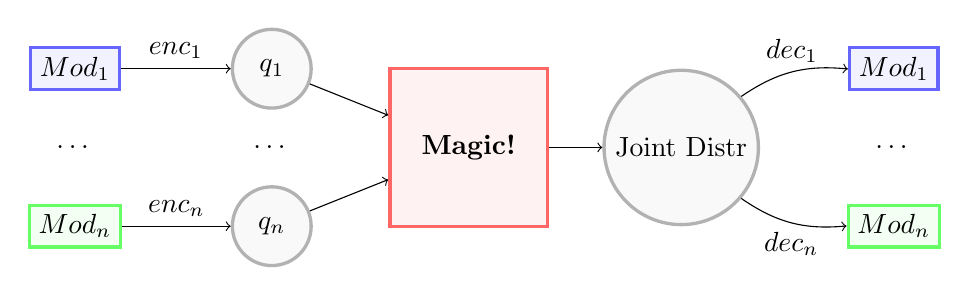
\begin{tikzpicture}[Mod1/.style={rectangle, draw=blue!60, fill=blue!5, very thick, minimum size=5mm},Mod2/.style={rectangle, draw=green!60, fill=green!5, very thick, minimum size=5mm},enc_mods/.style={circle, draw=gray!60, fill=gray!5, very thick, minimum size=10mm},magic/.style={rectangle, draw=red!60, fill=red!5, very thick, minimum size=20mm},]
                    \node[Mod1] (mod1) {$Mod_1$};
                    \node[below of=mod1] (points) {\ldots};
                    \node[enc_mods, right of=mod1, xshift=1.5cm] (q1) {$q_1$};
                    \node[Mod2, below of=points] (modn) {$Mod_n$};
                    \node[enc_mods, right of=modn, xshift=1.5cm] (q2) {$q_n$};
                    \node[below of=q1] (points) {\ldots};
                    \node[magic, right of=q1, yshift=-1cm, xshift=1.5cm] (magic) {\textbf{Magic!}};
                    \node[enc_mods, right of=magic, xshift=1.7cm] (joint) {Joint Distr};
                    \node[Mod1, right of=joint, xshift=1.7cm,yshift=+1cm] (rec_mod1) {$Mod_1$};
                    \node[right of=joint,xshift=1.7cm] (points) {\ldots};
                    \node[Mod2, right of=joint, xshift=1.7cm,yshift=-1cm] (rec_mod2) {$Mod_n$};
                    \draw[->] (mod1) -- node[anchor=south] {$enc_1$} (q1);
                    \draw[->] (q1) -- (magic);
                    \draw[->] (modn) -- node[anchor=south] {$enc_n$} (q2);
                    \draw[->] (q2) -- (magic);
                    \draw[->] (magic) -- (joint);
                    \draw[->] (joint) edge[bend left=20] node[anchor=south] {$dec_1$} (rec_mod1);
                    \draw[->] (joint) edge[bend right=20] node[anchor=north] {$dec_n$} (rec_mod2);
                \end{tikzpicture}
            }
        \end{figure}
    \end{frame}

    \begin{frame}{The Mixture-of-Products-of-Experts-VAE (MoPoE)}
        The MoPoE is a method from \cite{thomas_gener-ELBO}, which is a combination of:
        \begin{itemize}
            \item The Product-of-Experts (PoE) from \cite{wu2018multimodal}
            \item The Mixture-of-Experts (MoE) from \cite{shi2019variational}
        \end{itemize}
    \end{frame}

    \begin{frame}{The Mixture-of-Products-of-Experts-VAE (MoPoE)}
        \begin{figure}
            \centering
            \resizebox{0.9\textwidth}{!}{%
                \py{pytex_printonly(script='midterm_presentation/scripts/mopoe_graph.py', data = '')}
            }
        \end{figure}

        \begin{small}
            \begin{equation*}
                \log p_{\theta}(\mathbb{X}) \geq \eqlmopoe
            \end{equation*}

            \begin{equation*}
                \text{with:}\ \tilde{q}_{\phi}(\textbf{z}|\xsubset)=PoE(\{q_{\phi_j}(\textbf{z}|\textbf{x}_j) \forall \textbf{x}_j \in \xsubset\}) \propto \prod _{\textbf{x}_j \in \xsubset}q_{\phi_j}(\textbf{z}|\textbf{x}_j)
            \end{equation*}

        \end{small}

    \end{frame}

    \begin{frame}{Generalizing with the generalized $f$-mean}
        Both the PoE and the MoE can be generalized since both are special cases of the generalized f-mean \footcite{niculescu_convex_2018}:
        $$\mathcal{M}_{f}\left( \textbf{p} \right) = f^{-1}\left( \frac{1}{N} \sum ^N _{i=1} f(\textbf{p}_i)) \right)$$

        \textbf{Basic idea:}
        Make the fusion of the uni modal latent spaces more flexible by using an f-mean.
    \end{frame}

    \begin{frame}{Generalizing with the generalized $f$-mean}
        \begin{figure}
            \centering
            \resizebox{0.7\textwidth}{!}{%
                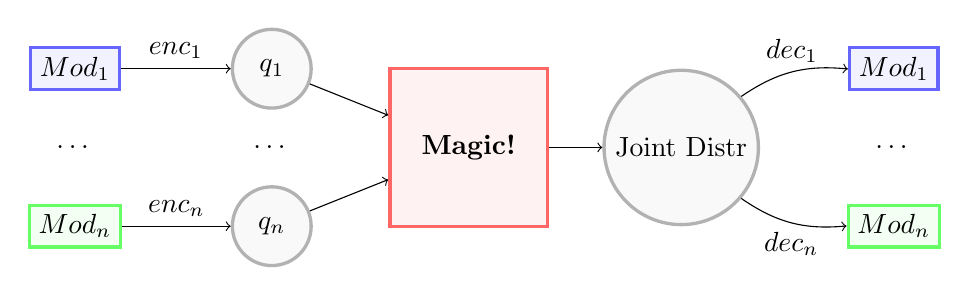
\begin{tikzpicture}[Mod1/.style={rectangle, draw=blue!60, fill=blue!5, very thick, minimum size=5mm},Mod2/.style={rectangle, draw=green!60, fill=green!5, very thick, minimum size=5mm},enc_mods/.style={circle, draw=gray!60, fill=gray!5, very thick, minimum size=10mm},magic/.style={rectangle, draw=red!60, fill=red!5, very thick, minimum size=20mm},]
                    \node[Mod1] (mod1) {$Mod_1$};
                    \node[below of=mod1] (points) {\ldots};
                    \node[enc_mods, right of=mod1, xshift=1.5cm] (q1) {$q_1$};
                    \node[Mod2, below of=points] (modn) {$Mod_n$};
                    \node[enc_mods, right of=modn, xshift=1.5cm] (q2) {$q_n$};
                    \node[below of=q1] (points) {\ldots};
                    \node[magic, right of=q1, yshift=-1cm, xshift=1.5cm] (magic) {\textbf{Magic!}};
                    \node[enc_mods, right of=magic, xshift=1.7cm] (joint) {Joint Distr};
                    \node[Mod1, right of=joint, xshift=1.7cm,yshift=+1cm] (rec_mod1) {$Mod_1$};
                    \node[right of=joint,xshift=1.7cm] (points) {\ldots};
                    \node[Mod2, right of=joint, xshift=1.7cm,yshift=-1cm] (rec_mod2) {$Mod_n$};
                    \draw[->] (mod1) -- node[anchor=south] {$enc_1$} (q1);
                    \draw[->] (q1) -- (magic);
                    \draw[->] (modn) -- node[anchor=south] {$enc_n$} (q2);
                    \draw[->] (q2) -- (magic);
                    \draw[->] (magic) -- (joint);
                    \draw[->] (joint) edge[bend left=20] node[anchor=south] {$dec_1$} (rec_mod1);
                    \draw[->] (joint) edge[bend right=20] node[anchor=north] {$dec_n$} (rec_mod2);
                \end{tikzpicture}
            }
        \end{figure}
    \end{frame}

    \begin{frame}{Generalizing with the generalized $f$-mean}
        \begin{figure}
            \centering
            \resizebox{0.7\textwidth}{!}{%
                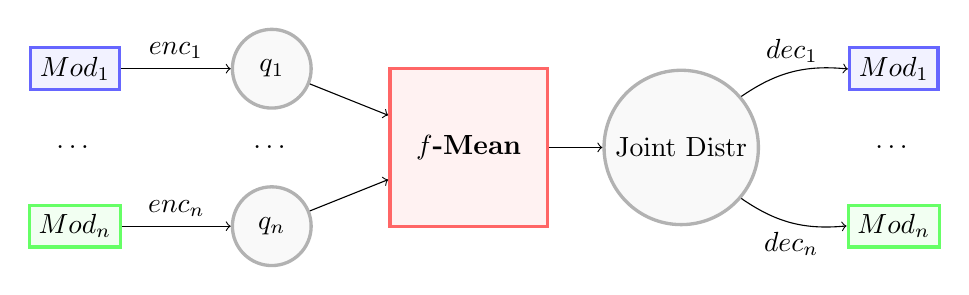
\begin{tikzpicture}[Mod1/.style={rectangle, draw=blue!60, fill=blue!5, very thick, minimum size=5mm},Mod2/.style={rectangle, draw=green!60, fill=green!5, very thick, minimum size=5mm},enc_mods/.style={circle, draw=gray!60, fill=gray!5, very thick, minimum size=10mm},magic/.style={rectangle, draw=red!60, fill=red!5, very thick, minimum size=20mm},]
                    \node[Mod1] (mod1) {$Mod_1$};
                    \node[below of=mod1] (points) {\ldots};
                    \node[enc_mods, right of=mod1, xshift=1.5cm] (q1) {$q_1$};
                    \node[Mod2, below of=points] (modn) {$Mod_n$};
                    \node[enc_mods, right of=modn, xshift=1.5cm] (q2) {$q_n$};
                    \node[below of=q1] (points) {\ldots};
                    \node[magic, right of=q1, yshift=-1cm, xshift=1.5cm] (magic) {\textbf{$f$-Mean}};
                    \node[enc_mods, right of=magic, xshift=1.7cm] (joint) {Joint Distr};
                    \node[Mod1, right of=joint, xshift=1.7cm,yshift=+1cm] (rec_mod1) {$Mod_1$};
                    \node[right of=joint,xshift=1.7cm] (points) {\ldots};
                    \node[Mod2, right of=joint, xshift=1.7cm,yshift=-1cm] (rec_mod2) {$Mod_n$};
                    \draw[->] (mod1) -- node[anchor=south] {$enc_1$} (q1);
                    \draw[->] (q1) -- (magic);
                    \draw[->] (modn) -- node[anchor=south] {$enc_n$} (q2);
                    \draw[->] (q2) -- (magic);
                    \draw[->] (magic) -- (joint);
                    \draw[->] (joint) edge[bend left=20] node[anchor=south] {$dec_1$} (rec_mod1);
                    \draw[->] (joint) edge[bend right=20] node[anchor=north] {$dec_n$} (rec_mod2);
                \end{tikzpicture}
            }
        \end{figure}
    \end{frame}

    \begin{frame}{Generalizing with the generalized $f$-mean}
        $f$ can be anything as long as it is injective
        $\rightarrow$ $f$ can be parameterized as a normalizing flow\footcite{papamakarios_normalizing_2019} $f_{\psi}$
        $$\mathcal{M}_{f_{\psi}}\left( \textbf{p} \right) = f_{\psi}^{-1}\left( \frac{1}{N} \sum ^N _{i=1} f_{\psi}(\textbf{p}_i)) \right)$$
    \end{frame}